\section{Controlling Mobile Traffic}
\label{sec:control}
In this section, we use two case studies to highlight some of the 
advantages \meddle provides as a new point of control 
for mobile networking traffic. We then discuss several new applications 
we are currently building.

\subsection{Packet Filtering}
Packet filtering is a common technique implemented in 
today's middleboxes. These can be used for implementing 
security policies, censoring content or preventing applications 
from harming the network (\eg, P2P). In \meddle, we use 
packet filtering to enable a number of features that are 
currently either unavailable or poorly implemented.

\noindent\textbf{Device-wide ad blocking.} Content and service providers 
typically use revenue from advertisements to cover their costs, enabling 
``free'' access for users. Given the additional costs in terms of data volume, 
battery consumption and potentially reduced privacy from tracking, it is unclear 
just how ``free'' these services truly are. Vallina-Rodriguez~\etal~\cite{Vallina-rodriguez:2012:AdCache} observe
that ads account for 5\% of daily traffic from more than 50\% of
Android users in a large European ISP. 

To understand the impact of ads using \meddle as a vantage point, we 
analyzed our traces and identified traffic for ads and analytics (A\&A) servers 
in terms of the portion of total traffic. Figure~\ref{fig:adblocking} presents our 
results. The x-axis represents users and the y-axis indicates the percent of 
total traffic generated by A\&A servers for all traffic and for only cellular traffic. 

We first observe that the amount of A\&A traffic per user is highly variable but can be 
significant. For example, the user with the largest total volume of traffic (user 1) saw 
54.25\,MB of ad traffic. The user with the largest portion of ad traffic (user 11) saw 
approximately 3\% of all traffic coming from A\&A servers, which corresponds to 8.3\,MB. 

Next, we observe that the amount of ad traffic can differ significantly 
based on whether the user is on cellular or not. Thus, a view of A\&A 
traffic that considers only cellular traffic can miss significant activity. 
To determine whether ad traffic differs across access technology, we use 
the following metric. First we find the ratio of a user's ad traffic over cellular 
to that over \wifi. Next, we find the ratio of a user's overall traffic over cellular 
to that over \wifi. We then take the ratio of the two, with the ad-traffic ratio 
in the numerator. If A\&A traffic were evenly distributed with non-A\&A traffic, 
we expect the ratio to be close to 1.

We include this ratio in parentheses in the figure. Users that do not have a cellular connection (tablets) have a value (-).
Most A\&A traffic occurs relatively evenly regardless of access technology (\ie, most of users have value in the range of 1).
For user 4, there is a clear exception. We were able to isolate this to a 
specific app using the request user agent. In this case, the we identified the traffic as 
coming from Niantic, a service that supports Google's Field Trip and Ingress apps. These 
are examples of augmented reality apps; we observe that their rising popularity could significantly 
impact users' data usage over cellular. 


\begin{figure}
\vspace{-2.5em}
\centering
        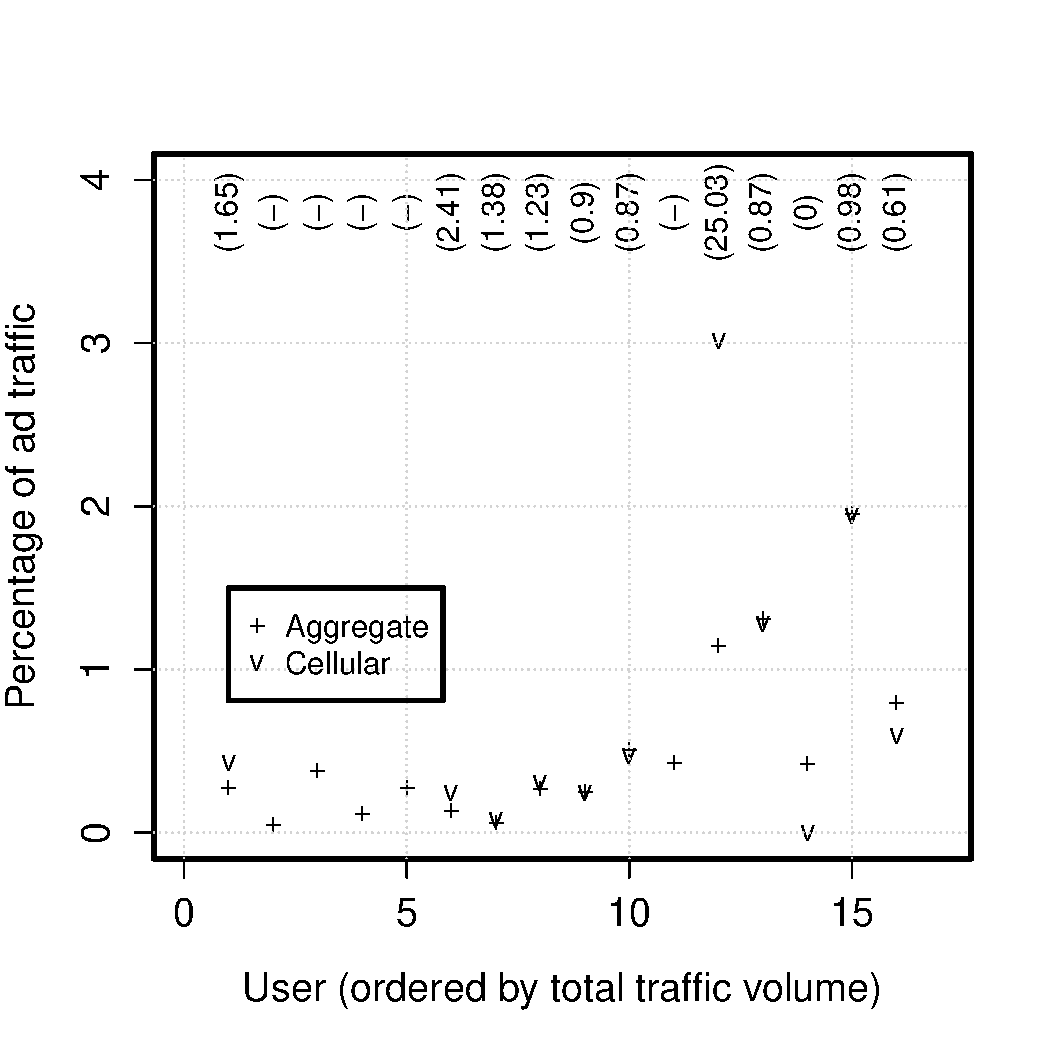
\includegraphics[width=\linewidth]{./plots/userAdsShare}
  \caption{Portion of user's traffic generated by ads and analytics (A\&A). A significant 
  portion of traffic (up to 3\%) comes from A\&A servers. For most users the A\&A 
  traffic occurs independently of access technology, but for some users it occurs 
  much more often on cellular than on \wifi. }
  \label{fig:adblocking}
   \vspace{\postfigspace}
\end{figure}


Our results, along with related work, highlight the fact that A\&A traffic can be 
significant. However, there is no current standard for opting 
out of unsolicited advertising; those that exist for tracking are not widely supported. 
Not surprisingly, many users have turned to software that blocks A\&A servers. 
For example, more than 20\,million users have installed 
AdBlockPlus~\footnote{http://www.adblockplus.org}, one of several tools for this purpose. 
Unlike the desktop environment, mobile device browsers do not provide support for 
ad blocking; further, most interactions occur inside of apps where browser plugins 
cannot help. 

\meddle makes it easy to implement an efficient, device-wide ad blocker. 
In our current implementation, we use a DNS-based filter to
block ads, analytics, and mediation sites.\footnote{The service is disabled by default, so users must 
opt in to enable blocking.} A key feature of our solution is that it works 
regardless of whether SSL is used because DNS requests occur out of band 
from the secure connection. Further, the response for the DNS request is an IP address corresponding to {\tt localhost}, 
meaning that devices will generate no external network traffic when failing 
to resolve the ad servers. 


Our ad blocking engine relies on a publicly available list of domains for A\&A servers~\cite{YoyoAds}; we augment this list of domains using 
recent research on mobile ads~\cite{hornyack:appfence,
  Leontiadis:2012:AdsMobile}. From our initial deployment, we observed a 0.05\% to 3\% reduction
in total traffic at each mobile device due to our ad blocking engine. 
In addition to the DNS-based filter, we are currently implementing a filter that blocks 
requests for URLs matching a regular expression, as done by AdBlockPlus.

Finally, we note that wholesale blocking of advertisements may be considered harmful 
to the long-term viability of services that do not charge fees. In Section~\ref{subsec:newapps}, 
we discuss an alternative model that incorporates a Privad proxy implemented as a meddlebox. 

\noindent\textbf{Do not disturb.} 
Many users do not turn off their devices at night, even while asleep. In our study, we found that 
most (89\%) of the devices were active for at least one entire 24-hour period. Network 
traffic occurring during those periods is generally not helpful for the user; worse, 
such traffic may cause audible alerts that wake up the user. In part to address this, 
iOS 6 introduced a ``Do not disturb'' feature that silences the phone and \emph{reduces} 
network activity. We are unaware of such support on Android.

\meddle enables a cross-platform and cross-device ``Do not disturb'' for network 
traffic. Users specify the hours when traffic should be blocked and the corresponding 
meddlebox will drop all traffic. Further, users can specify hosts that should \emph{not} be 
blocked. An interesting area of future work is to map apps to their network-traffic 
signatures, enabling users to specify per-app policies via \meddle.

\noindent\textbf{Content Restrictions.} 
Existing controls for restricting access to content from mobile devices (\eg parental controls) 
tend to focus on which apps a user cannot run. For example, a parent can block the Facebook app on an iOS device. 
To the best of our knowledge, there is no way to prevent a user from using a 
Web browser to access the Facebook site, unless all Web browser activity is blocked. 

In general, this would be too prohibitive. Using \meddle, we can blacklist traffic for 
all IPs known to belong to a content or service provider. For example, to block 
Facebook we would block IPs belonging to Facebook, as well as any traffic using Facebook 
SSL certificates (\eg, for accessing content hosted by CDNs). 

\subsection{Traffic Manipulation}
An advantage of \meddle is that it provides isolation from carriers' in-network 
middleboxes, which may block, modify or shape certain network traffic. However, 
toward the goal of improving transparency in mobile networks (especially for 
non-\meddle users), we would like to be able to identify when, how and what 
network traffic is subject to carrier manipulation. 

In this section, we describe how we use \meddle to detect HTTP interference via 
in-flight Web page changes. We believe our technique 
is general to other protocols. 

The problem of HTTP interference was highlighted 
by Reis et al.~\cite{reis:tripwires}. The authors demonstrated that although a small 
precent of users were affected by in-flight changes, those changes tended to introduce 
vulnerabilities such as overflows and cross-site scripting (XSS) attacks. They proposed and deployed 
\emph{Web Tripwires}, Javascript code that detects in-flight page changes. The main 
limitation of their study is that the approach requires each Web site to modify their content to 
include a tripwire.

\noindent\textbf{Web Tripnets.} Using \meddle, we extended tripwires to alleviate this 
limitation. Namely, we use \meddle to inject a tripwire on \emph{any} page without requiring 
support from Web site developers -- an approach we call a \emph{Web Tripnet}.

When enabled, the Web tripnet works as follows (depicted in Fig.~\ref{fig:tripnet}). First, the device requests a Web page via 
HTTP (1). Because the \meddle connection is encrypted, the device's 
provider cannot alter the page in flight. When the Web server response arrives at 
the \meddle server (2), we insert a Web tripwire before forwarding the response to the user. 

To detect whether the carrier would have manipulated the 
page without \meddle, we create a \emph{pigeonhole} by configuring the device's VPN settings to send 
traffic for a particular site in the clear. When the Web tripwire attempts to load another copy 
of the Web page (3), the request is redirected (using DNS) to a transparent proxy that forwards the request to the intended server, 
retrieves the Web page and delivers it to the device in the clear (thus exposing it to carrier manipulation). 
Upon receiving the page over an unencrypted channel, the device's browser sends both 
versions of the Web page (tunneled and untunneled) to the \meddle server for analysis. 

\begin{figure}
\centering
        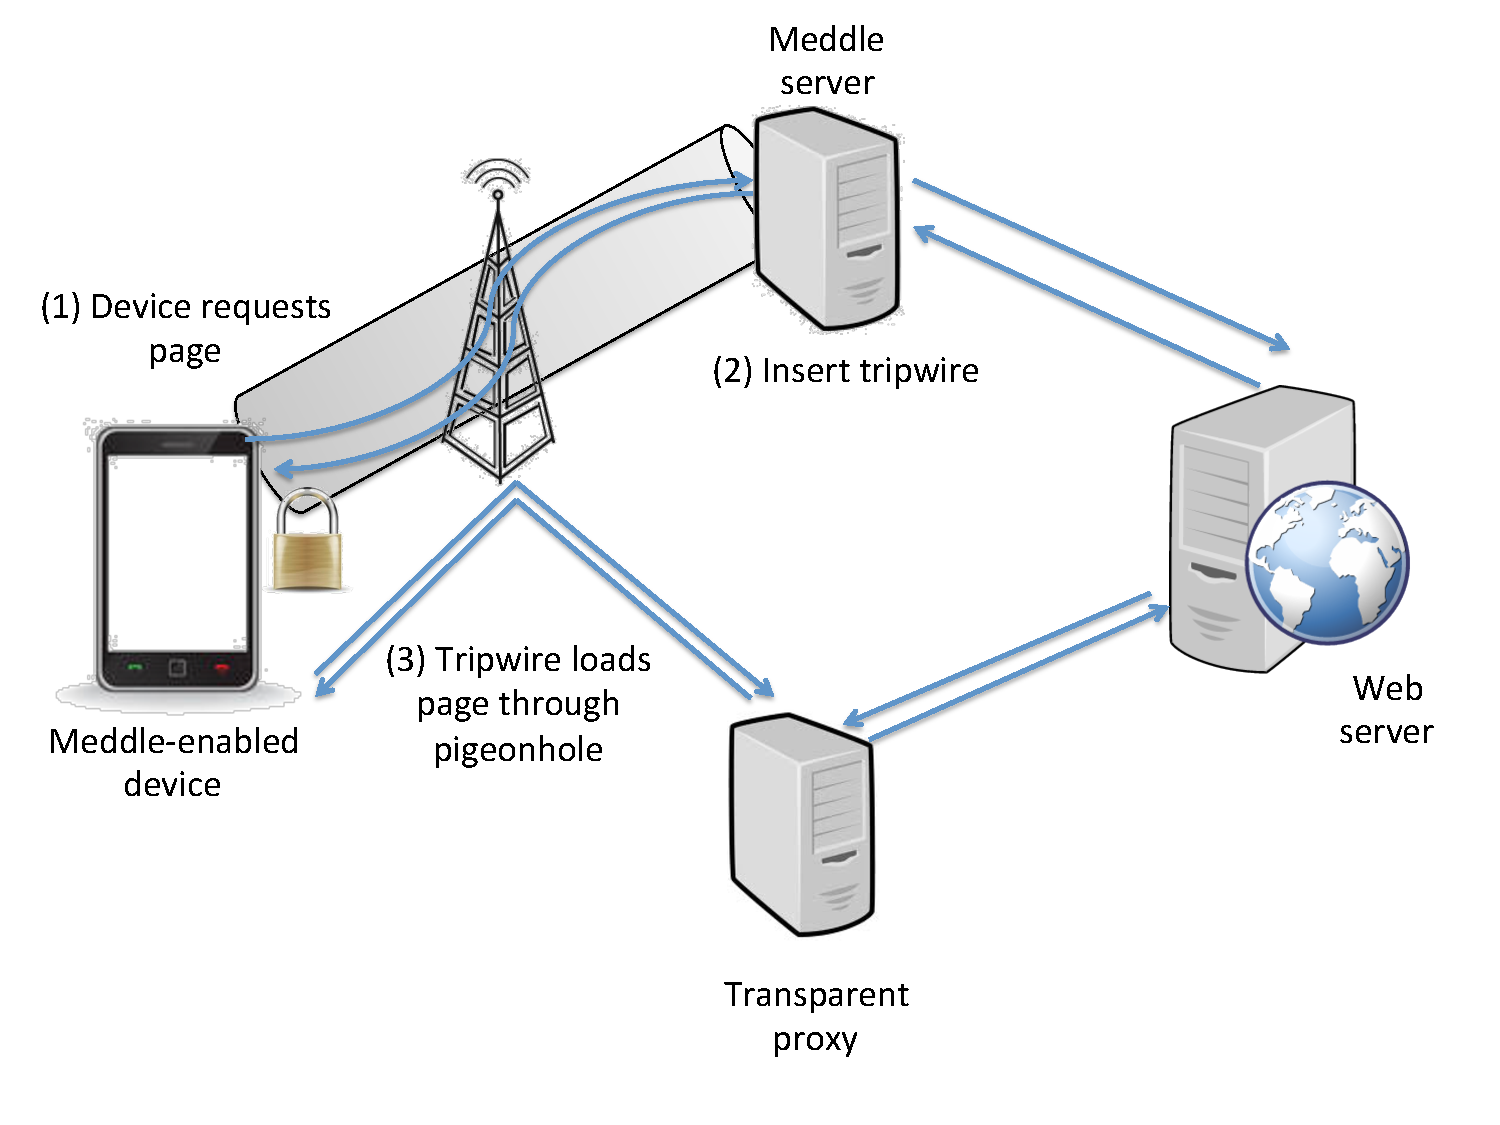
\includegraphics[width=\linewidth]{figs/tripnet.pdf}
\vspace{\figcapspace}
  \caption{Overview of the \meddle Web tripnet. A Web page is loaded 
through the VPN tunnel, where a meddlebox inserts a Web tripwire. The 
tripwire causes the browser to reload the Web page using the address of a
transparent proxy server that is accessed using an unencrypted connection. 
After the proxied version of the page is loaded, a message is sent to the user if 
the pages differ due to ISP interference. }
  \label{fig:tripnet}
\vspace{\postfigspace}
\end{figure}

\noindent\textbf{Experimental Results.} We conducted a survey of HTTP manipulation using two US carriers (Verizon and T-Mobile) 
and one French carrier (Orange). To determine if the user agent can impact manipulation from 
carriers, we tested using Android, iOS and a desktop (tethered) browser. We tested the top 
100 sites according to Alexa, in addition to a random sample of 100 of the 10,000 most popular 
sites. Our analysis did not identify any carrier manipulation. This is not entirely surprising, 
since most manipulation identified by Reis et al. occurred due to software installed inside 
a user's network.

An interesting observation is that 
we found one example where Facebook over Verizon included a promotional link specific to 
Verizon, even when the connection was proxied through a host at the University of Washington. 
Further analysis showed that the Squid proxy's {\tt X-Forwarded-For} field was being populated 
with an address in Verizon's network, and Facebook was modifying the page accordingly. When 
we removed the {\tt X-Forwarded-For} field, the promotional link no longer appeared. 

\subsection{New Applications}
\label{subsec:newapps}

\meddle allows researchers to explore the space of applications that offload 
networking traffic from mobile devices to a server where power and data quota 
are less scarce. We envision several important applications that can benefit 
from our approach.

\begin{packeditemize}
\item \textbf{P2P offloading.} P2P services tend to benefit from multiple connections 
and symmetric bandwidth contributions from participating hosts. Both of these are 
costly in the mobile environment. \meddle can ease these costs by offloading the 
logic for maintaining P2P connections to a meddlebox.
\item \textbf{Privad.}  Instead of simply blocking ads, \meddle is an ideal location 
to deploy anonymizing systems that support targeted advertising, as suggested by 
Guha et al.~\cite{guha:privad}. This can alleviate concerns for user privacy and can 
serve as a viable alternative to wholesale ad blocking.
\item \textbf{Tor.} \meddle improves privacy in mobile networking by encrypting the 
connection from the mobile device to the \meddle server. We can further improve 
privacy and anonymity by providing a Tor meddlebox that establishes and manages 
onion-routed connections.
\item \textbf{Privacy Preserving Photo Sharing.} Recently Ra et al~\cite{ra:p3} propose 
using indirection to support privacy-preserving photo-sharing for mobile users. \meddle 
provides an ideal vantage point from which to deploy this service without requiring 
users to install additional apps. 

\end{packeditemize}


%Example Apps (highlight things we can do with meddle)
% - Begin with a sentence/intro-para on using middleboxes to offloading activities and offer device wide services
% - Middlebox based packet monitoring 
%      - cross * possible
%      - passive - real traffic 24x7 
%      - actual users
%      - Network traffic characterization
%         - Longitudinal study of network traffic
%         - understand behavior of apps
% - Device wide services - service like packet filtering that is not limited to an app 
%     - Ad blocking
%     - Platform for malware detection and blocking
%     - Parental controls 
% - Deployment of new protocols and services 
%   - Users can opt in for specific service
%   - Mobile story for services like FreeDOM, CCNs, etc.
%   - service in a VM where users opt in for services
% - Generic Proxy
%   - Privad
%   - Anti-censorship